
%\section{Data Overview} 

 
ZI's to do... 

\subsection{Stripe 82 dataset} 

ZI: why S82, what we used, data size...


\subsection{The treatment of seeing in SDSS}

ZI: steal the relevant text from the EDR paper (\citet{SDSSEDR}) and photo papers by \cite{Lupton2001} 
and \cite{Lupton2002}. 


\subsubsection{QA plots from SDSS Postage Stamp Pipeline (PSP)}

Testing (will probably be removed later): for each run, camera column and filter, PSP makes three QA plots, 
Figs.\ref{fig:PSPplot1}--\ref{fig:PSPplot3}. 


\begin{figure}
\centering
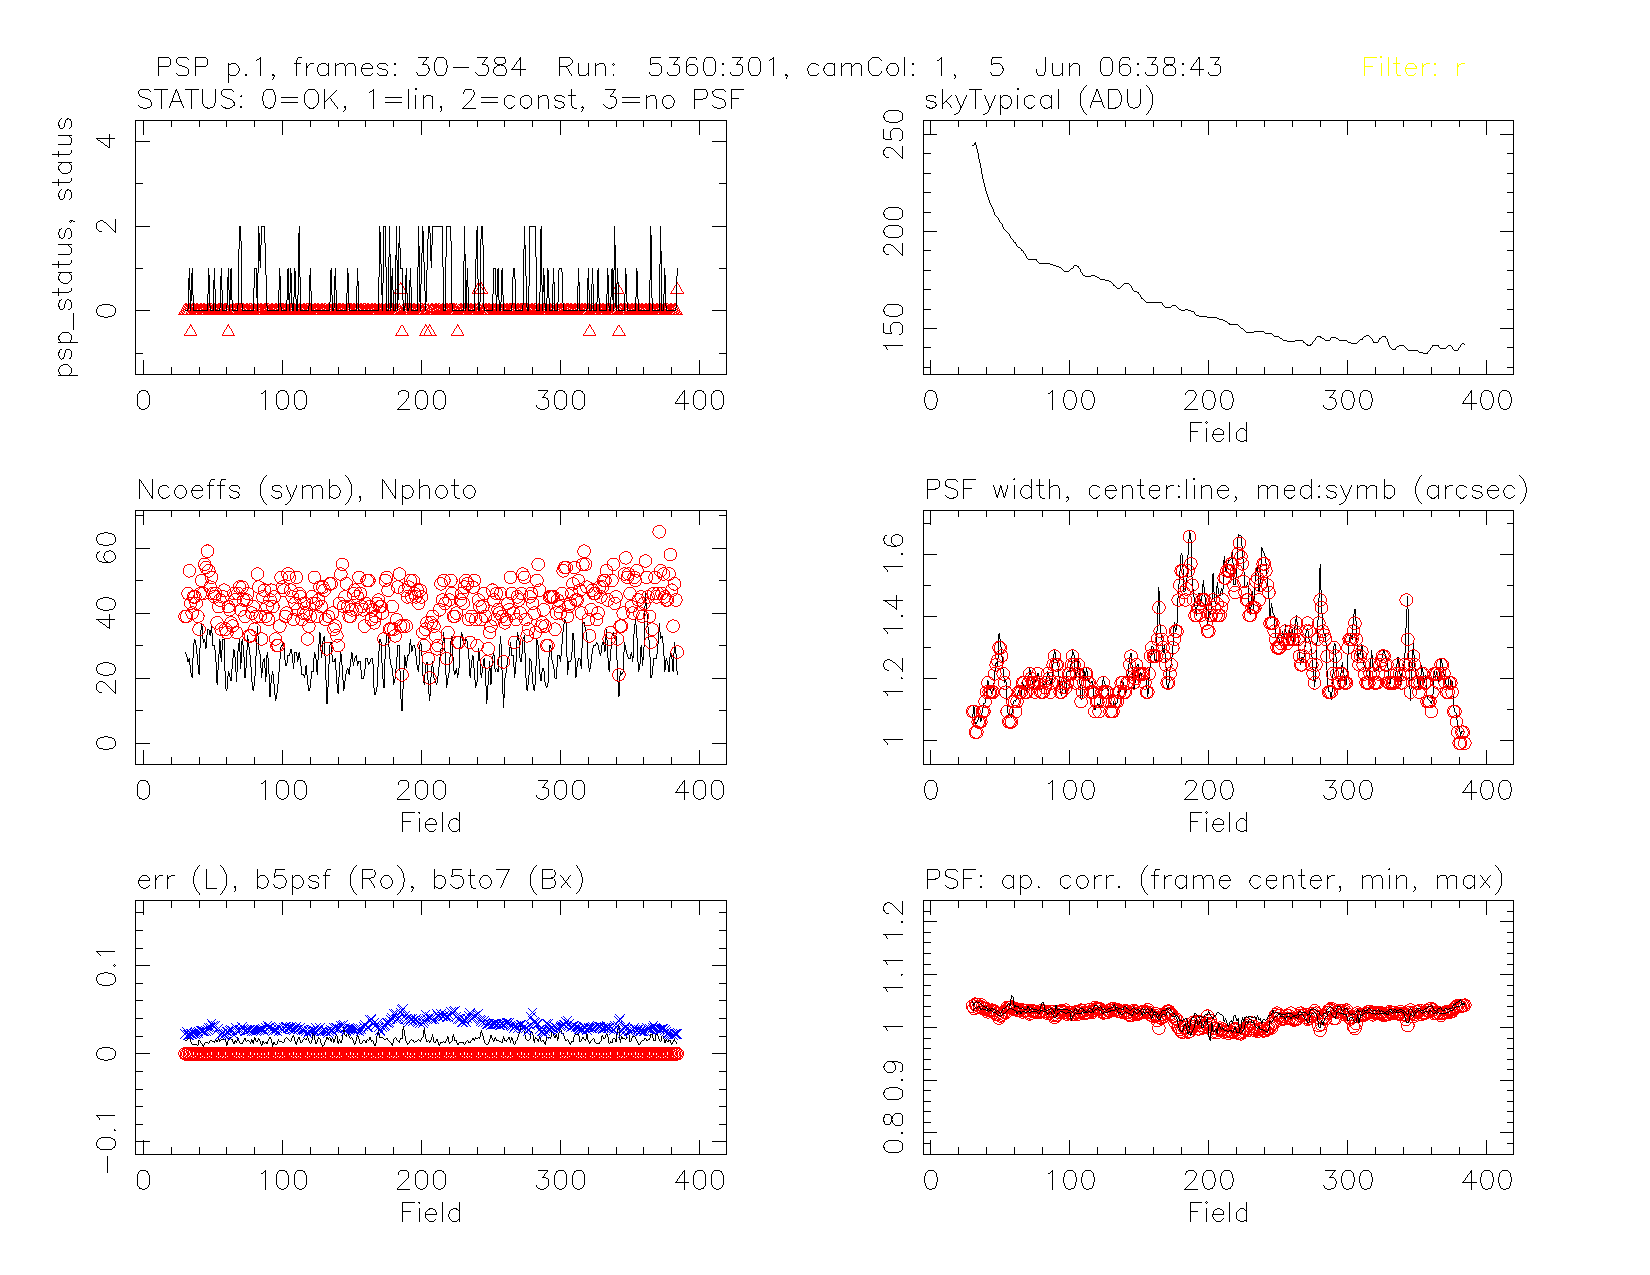
\includegraphics[width=0.9\textwidth]{FIGURES/psPlots1-005360-r1.pdf}
\caption{The plot 1 (psPlots1-005360-r1) produced by PSP for SDSS run 5306, 
camera column 1, in the $r$ band. The middle right panel shows the FWHM for
the measured seeing, as a function of field number (that is, as  function of time, 
with one field cooresponding to about 36 seconds). Note the large deterioration
of seeing between fields 130 and 300, lasting a bit under 2 hours. 
\label{fig:PSPplot1}}
\end{figure}


\begin{figure}
\centering
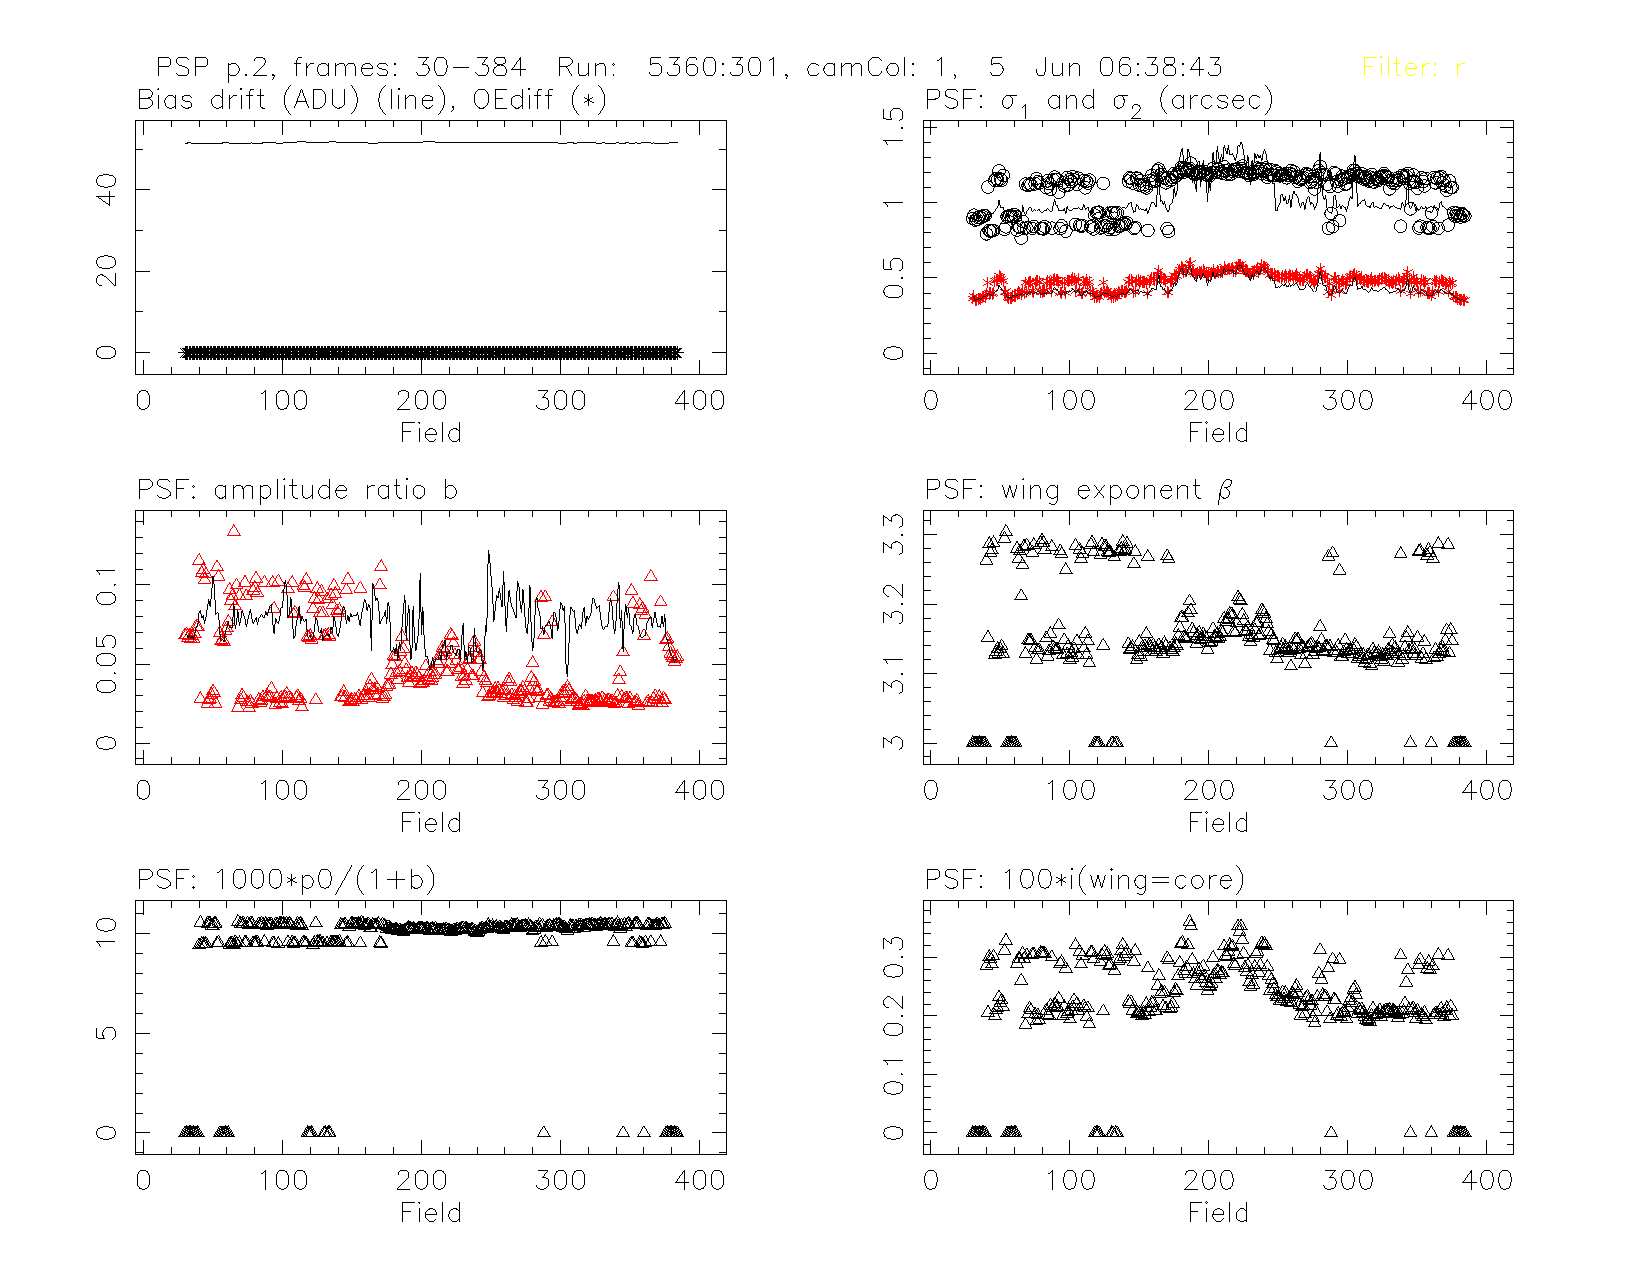
\includegraphics[width=0.9\textwidth]{FIGURES/psPlots2-005360-r1.pdf}
\caption{Similar to Fig~\ref{fig:PSPplot1}, except that here the plot 2 is shown.
Except for the top left panel, the best-fit PSF parameters (a double Gaussian
plus a power-law wing) are shown (see text for their description). 
\label{fig:PSPplot2}}
\end{figure}


\begin{figure}
\centering
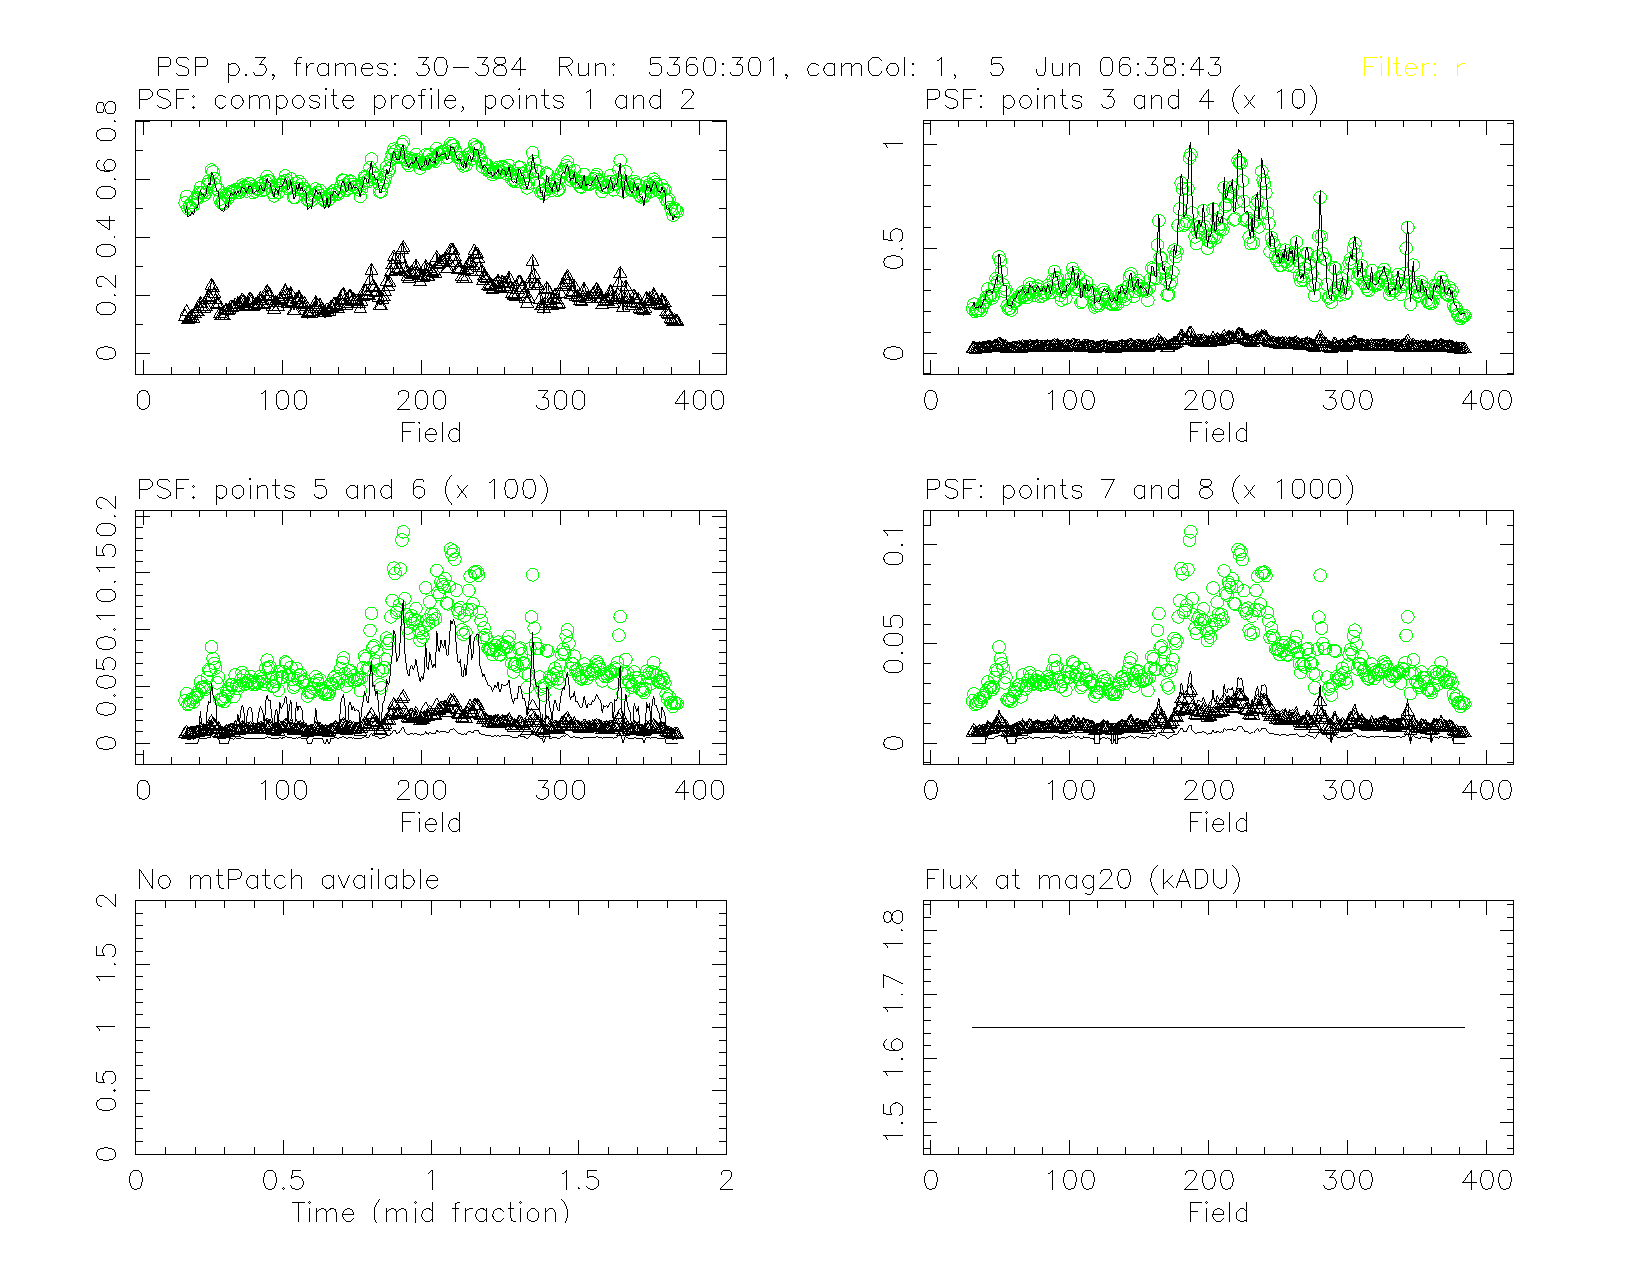
\includegraphics[width=0.9\textwidth]{FIGURES/psPlots3-005360-r1.pdf}
\caption{Similar to Fig~\ref{fig:PSPplot1}, except that here the plot 3 is shown.
The top four panels show the values of composite PSF profile (data).
\label{fig:PSPplot3}}
\end{figure}
